\documentclass[12pt,letterpaper,noanswers]{exam}
%\usepackage{color}
\usepackage[usenames,dvipsnames,svgnames,table]{xcolor}
\usepackage[margin=0.9in]{geometry}
\renewcommand{\familydefault}{\sfdefault}
\usepackage{multicol}
\pagestyle{head}
\usepackage{hyperref}
\definecolor{c07}{HTML}{BBFFBB}
\definecolor{c08}{HTML}{BBFFFF}
\definecolor{c09}{HTML}{BBDDFF}
\definecolor{c10}{HTML}{BBBBFF}
\definecolor{c11}{HTML}{DDBBFF}
\definecolor{c12}{HTML}{BBBBDD}
\newcommand{\mb}[1]{\underline{#1}}

\header{AM 22b Problem Set 06}{}{Due Thurs Mar 25th at 6pm}
\runningheadrule
\headrule
\usepackage{diagbox}
\usepackage{graphicx} % more modern
%\usepackage{subfigure} 
\usepackage{amsmath} 
\usepackage{amssymb} 
%\usepackage{gensymb} 
%\usepackage{natbib}
\usepackage{hyperref}
%\usepackage{enumitem}
%\setlength{\parindent}{0pt}
%\usepackage{setspace}
%\pagestyle{empty}  
%\newcommand{\Sc}[0]{
%{\color{BlueViolet}\S}
%}
\usepackage{tcolorbox}

\begin{document}
 \pdfpageheight 11in 
  \pdfpagewidth 8.5in

\begin{questions}
\question Log in to WeBWorK and complete the problems assigned there under pset06.




\item In the Atlantic Ocean off the coast of Newfoundland, Canada, the temperature and salinity (saltiness) vary throughout the year.  The figure below shows a parametric curve giving the average temperature, $T$ (in $^\circ$C) and salinity (in grams of salt per kilogram of water) for $t$ in months, with $t=1$ corresponding to mid-January.
\begin{parts}
\item Why does the parameterized curve form a loop?
\begin{solution}
The data is periodic in time.  It is the average temperature and salinity in each month, and January immediately follows December.
\end{solution}
\item When is the temperature highest?
\begin{solution}
The temperature is highest in month $8$, which is mid-August.  $t=1$ corresponds to January, and the temperature then gets colder in February and March, warms slightly in April and May, and warms substantially in June and July before peaking in August.
\end{solution}
\item When in the water saltiest?
\begin{solution}
The water is saltiest in April (just a little saltier than March) since that is when the salinity value is largest.
\end{solution}
\item Use a local average value to estimate the instantaneous rate of change of the temperature with respect to the salinity at $t=6$ and give the units.
\begin{solution}
To approximate the instantaneous rate of change of temperature with respect to salinity in June, use the average value between May and July (or the average between May and June or the average between June and July).  The change in salinity from May to July is about $-0.25$ grams per kilogram.  The change in temperature is about $4.5$ $^\circ$C.  We have $\Delta T/\Delta s \approx -4.5/0.25 = -18$ $^\circ$ C per (gm/kg).  The units are degrees C per gm/kg or $^\circ$C kg/gm.
\end{solution}
\end{parts}
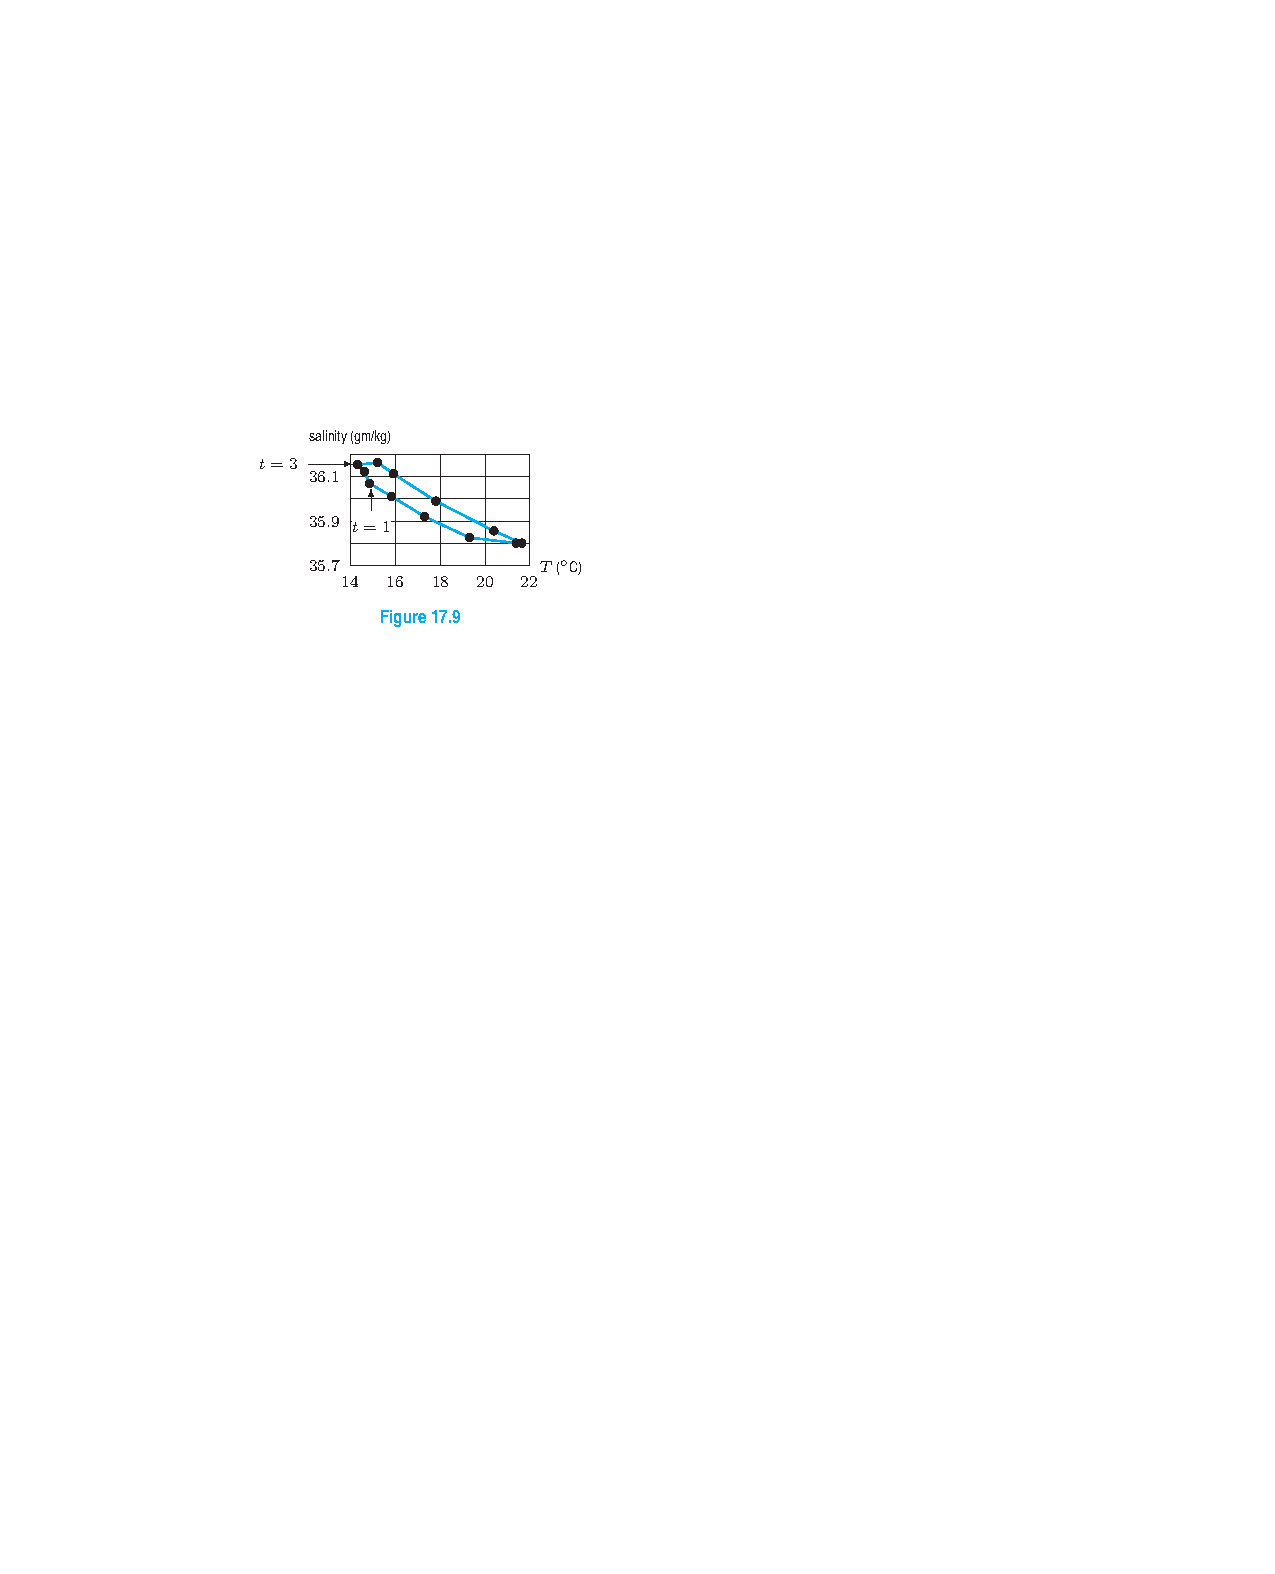
\includegraphics{img/HW08p1.pdf}

\question The function $f(x,y,z)$ is defined and smooth at every point in $3$-space.  $\left.\nabla f\right\vert_{(1,7,2)} = \langle 1,-\sqrt{6},1\rangle$.  A curve $C$ is given by $\mb r(t) = (t+1)^2\mb i + 7\cos t\mb j + 2e^t\mb k$.



\begin{parts}
\item Find a parameterization for the line perpendicular to the level surface at $(1,7,2)$.  Show your mathematical reasoning.
\item Find an equation for the tangent plane to the level surface of $f$ at $(1,7,2)$.
\item Find the angle between a normal vector to the level surface of $f$ and a tangent vector to the curve $C$ at $(1,7,2)$.  Choose the smaller of the two possible angles (and give your answer in radians).
\item Assume $x,y,z$ are in centimeters.  Let $f$ represent the concentration of a pollutant, in parts per million, at the point $(x,y,z)$.  A particle moves along the curve $C$ with the given parameterization (with $t$ in seconds).  Find the instantaneous rate of change of the concentration with time when $t = 0$ s.  Include units in your answer.
\end{parts}


\question (A connection between $e$ and $\pi$).  

A Gaussian function in one variable is a function $f(x) = ke^{-(x-x_0)^2/(2b^2)}$.  

 The Gaussian function is the basis of an important probability density function called the \textbf{normal} distribution.   Consider a two-dimensional version, $f(x,y) = k e^{(-x^2-y^2)/2}$.  For this to be a probability density function, we would need $\int_{-\infty}^\infty\int_{-\infty}^\infty f(x,y)\ dx\ dy = 1$.    You found $k$ so that $f(x,y)$ is a probability density function on a previous problem set by working analytically.


We will also use Monte Carlo integration to approximate the value of $k$.  


\begin{parts}
    \item
Estimate $\displaystyle I = \int_{-B}^B\int_{-B}^B e^{(-x^2-y^2)/2}\ dx\ dy$ using Monte Carlo integration, choosing increasing values of $B$.  Work to find an estimate of $I$ to two decimal places.

\item
Submit a screenshot of your \texttt{Matlab} code on Gradescope for this as part of your problem set submission.

\item Once you've approximated $I$, provide an approximate value of $k$.

We say a function has \textbf{bounded support} if the function is nonzero on a bounded region of the $xy$-plane.  When a function has bounded support, we can enclose the bounded region within a box to use Monte Carlo integration.

Our function does not have bounded support, but the value of the function is decreasing rapidly away from the origin, so most of the contribution to the integral will come from the region around the origin.

\end{parts}





\question (parameterized path) A person has a $0.4$ m long baton with a light on one end.  They throw the baton so that it moves entirely in a vertical plane.  To describe the plane, choose an origin on the ground and let the $y$-axis point vertically.

\begin{itemize}
\itemsep0em
    \item The center of the baton follows a parabola.
    \item The baton rotates counterclockwise around its center (with constant angular velocity, so a constant rate of rotation).
    \item The baton is initially horizontal and $1.5$ m above the ground.
    \item Its initial velocity is 8 m/sec horizontally and 10 m/sec vertically.
    \item Assume there is downward acceleration due to gravity (approximate its magnitude as $9.8$ m/s$^2$), and no other acceleration.
    \item Its angular velocity is 2 revolutions per second.

\end{itemize}
Find parametric equations describing
\begin{parts}
\part  the motion of the center of the baton relative to the ground.
\part the position of one end of the baton relative to its center
\part the path traced out by the end of the baton relative to the ground.
\part Use matlab to plot the motion of the center of the baton and the end of the baton (on the same axes).
\end{parts}

\question For each of the following functions
\begin{itemize}
    \item Describe the level surfaces in words.
    \item Find the gradient (as a function of position).  This is a vector field in $3$-space.  Where appropriate, use $\mb r$ in your expression for the gradient field.
    \item Describe the vector field in words.  Is it radial?  parallel to an axis or to a plane?  is the magnitude increasing, decreasing, or constant moving away from the origin? etc.
\end{itemize} 

\begin{parts}
\part $x^2+y^2+z^2$
\part $\sqrt{x^2+y^2+z^2}$
\part $3x + 4y$
\part $3x + 4z$
\end{parts}

\question (flow lines) Let $H(x,y)$ be a smooth function (so that its partial derivatives are defined and are smooth).  Let $\mb v = -H_y\mb i + H_x\mb j$.
\begin{parts}
\part 
 Show that $\mb v$ is perpendicular to $\nabla H$ at each point $(x,y)$.
    \item Show that the flow lines of $\mb v$ sit along level curves of $H$.

\end{parts}


\end{questions}

\end{document}
